\section{Visualization}\label{sec:visualization}

\begin{table}[h]
    \caption{Relationship between charts and ER-tables.}
    \centering
    \begin{tabular}{ll}
        \toprule
        ER-Table & Chart             \\
        \midrule
        Battles  & Geographic Map    \\
                 & Line Chart        \\
                 & Stacked Bar Chart \\
                 & Scatter plot      \\
        Wars     & Box Plot          \\
        \bottomrule
    \end{tabular}
\end{table}

\subsection{Geographic Map}
The first component of our visualization tool is the geographic map, whose goal is to show to the end customer the precise projected point (using longitude and latitude attributes) where a particular battle occurred. In particular, we took an European continent picture with its respective countries boundaries information, and projected the real battles coordinates over it, in order to properly fit them to our figure. We represented each battle with a clickable circle, whose color depends on the battle outcome (e.g. won, lost, \dots). In order to improve the quality of the analysis, we offer the possibility to know some details about the currently selected battle: indeed, we have provided a small legend which summarizes some useful information such as battle name, the year, the coordinates and its outcome. Furthermore, it is possible to select multiple battles via the brushing approach. In fact, when a number $n > 2$ of battles is selected, the legend will show that $n$ battles have been selected and also the range (of years) in which they have been occurred. Note that, when brushing, the unselected battles are hidden.

\begin{figure}[h]
    \centering
    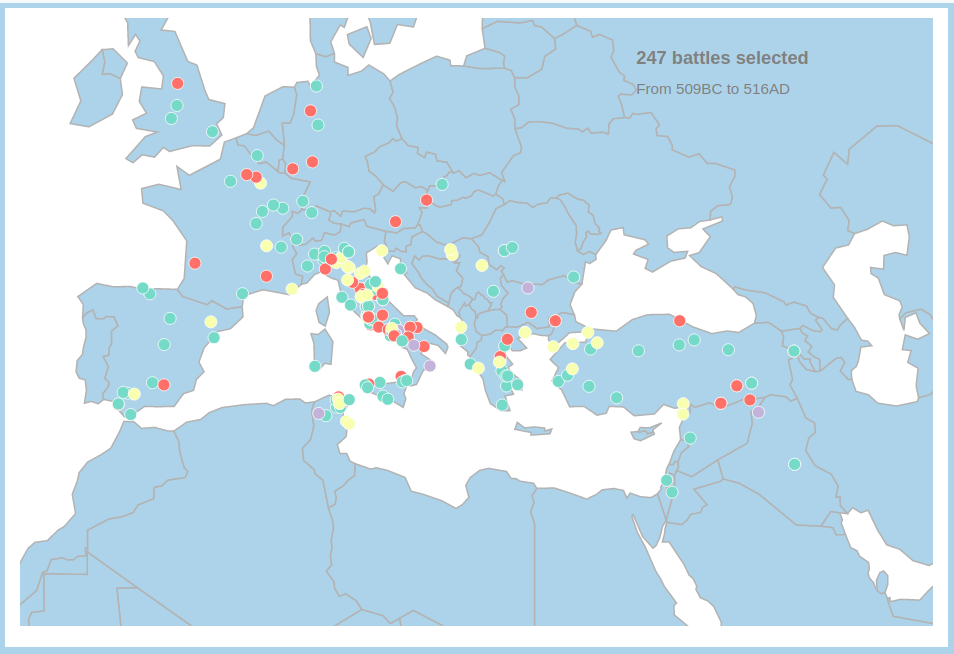
\includegraphics[scale=0.20]{./images/geographic_map.png}
    \caption{Geographic map}
\end{figure}

In this scenario, the other charts of the visualization will be properly updated. Conversely, also the geographic map will be updated when a particular time period is selected in the Line chart or a group of battles is selected in the Scatter plot. In the first case, the battles outside the selected time period are hidden, whereas in the second scenario the selected battles are highlighted with a black border.

\subsection{Infobox}
In order to allow the end customer to explore further information about a specific battle, we have implemented an information container, using Bootstrap modal feature, that will be shown to him when he will click on the marker of a battle. 
\begin{figure}[H]
	\centering
	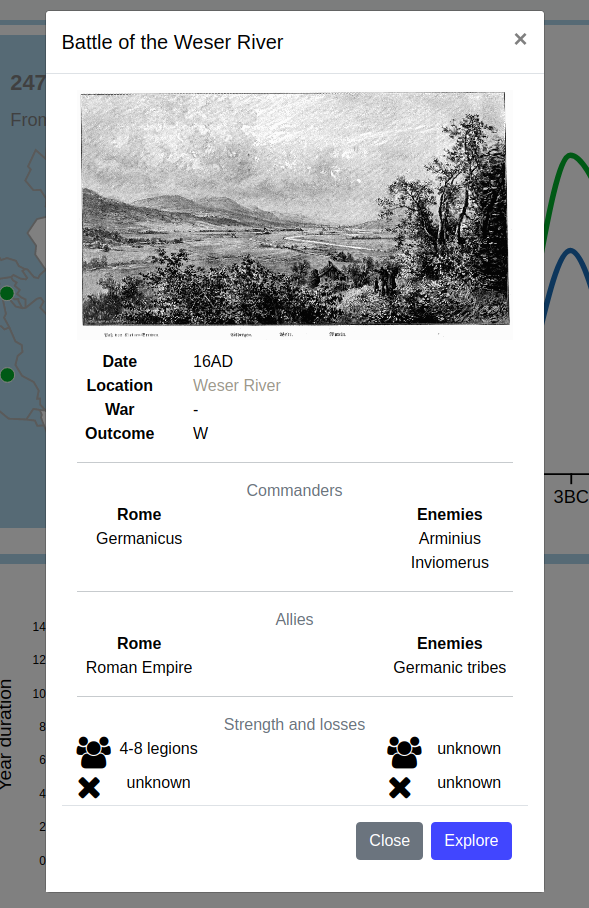
\includegraphics[scale=0.20]{./images/infobox.png}
	\caption{Infobox example}
\end{figure}
In this container we can find the image of the battle if present, otherwise it will be shown a placeholder, the battle data, location, war and outcome. If the corresponding location has the pleiades identifier, then it will be clickable to explore more information about it. Furthermore, we can find the commanders of the Roman and enemies empire, as well as their allies. At the end of the container, we can find some statistical measures about the strength and losses of the two counterparts. The last thing we want to underline is the possibility to explore further war details of the chosen battle through the button Explore, if and only if the corresponding war identifier is present.
\subsection{Line Chart}
The next component is the Line chart, which is responsible to communicate to the analyst the trends of won and lost battles in a given time period. We provided two analysis approaches:
\begin{itemize}
    \item \textbf{by centuries} in order to analyze the previous trends from a general point of view in century form
    \item \textbf{cumulative}, which allow us to perform a more specific analysis with respect to the previous one, taking into account the trends in year form.
\end{itemize}

\begin{figure}[h]
    \centering
    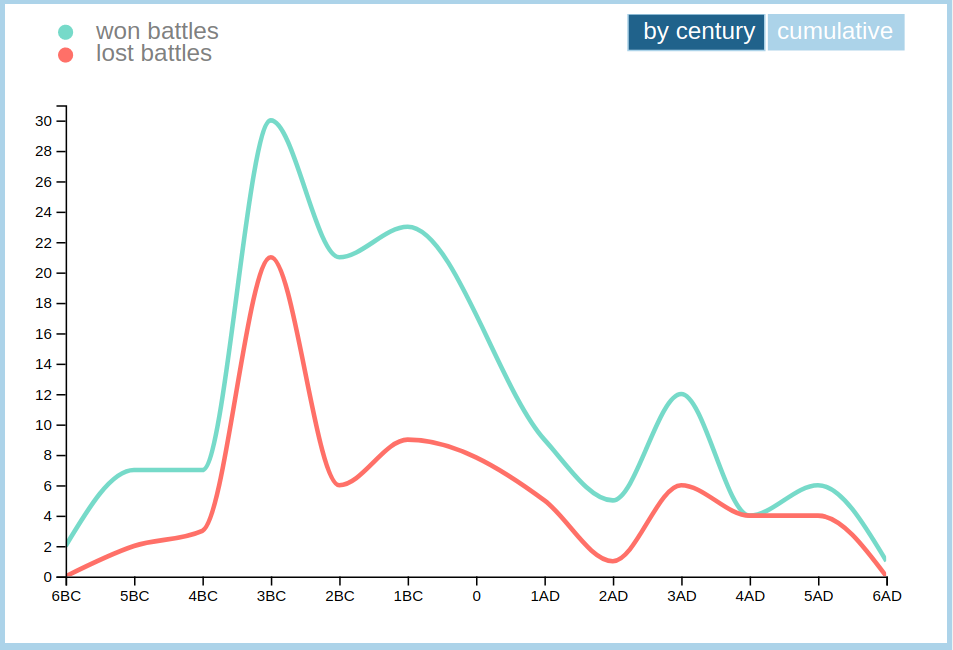
\includegraphics[scale=0.20]{./images/line_chart.png}
    \caption{Line chart showing century by century the number of battles.}
\end{figure}

The Line chart has two main axes: the $x$ axis represents centuries or years, and the $y$ axis represents the number of battles. The first interaction on this chart is reached through brushing plus zooming approach. In fact, selecting a specific time period via brushing, the zoom function will update the chart axis's ranges and data. To remove a selection, the user has just to perform a double click. In this scenario, the selected data will update also the geographic map, the stacked bar chart and the scatter plot. On the contrary, this chart will be updated if only if any change occurs in the geographic map.

\subsection{Stacked Bar Chart}
\begin{figure}[h]
    \centering
    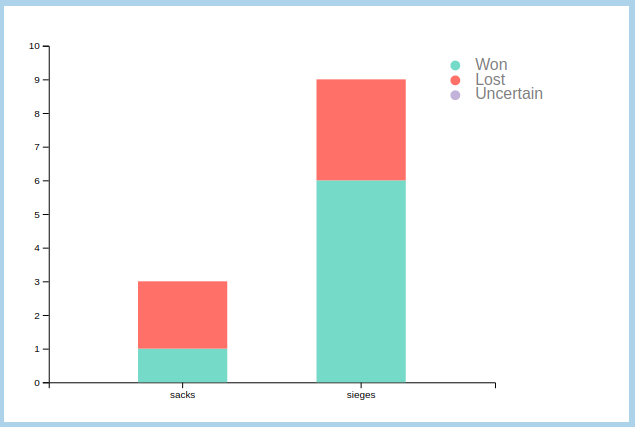
\includegraphics[scale=0.30]{./images/stacked_bar_chart.png}
    \caption{Stacked Bar chart}
\end{figure}
The stacked bar chart is another component of our visualization that offers a different type of analysis. It's constituted by two axes: the $x$ axis represents two battle types: \textbf{sacks} and \textbf{sieges}; the $y$ axis, instead, represents the number of the battles. This analysis is based on won, lost and uncertain battles (as usual we reported a legend for reasons of clarity).

This chart is not able to update the other ones, but can be updated with a selection performed in the geographic map, in the line chart or over both of them.

In case of doubts about the actual number of battles outcome with a particular type, the user can simply move the mouse pointer over that specific layer, thus producing a small label (tooltip) showing the exact number: this can be extremely useful because of the intrinsic nature of the stacked bar chart and its bars displayed one on top of the other.


\subsection{Box Plot}
\begin{figure}[h]
    \centering
    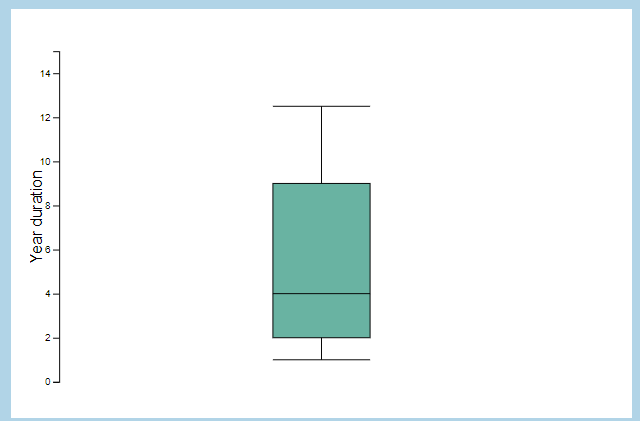
\includegraphics[scale=0.5]{./images/box_plot.png}
    \caption{Box plot}
\end{figure}
The Box Plot is another component of our visualization tool: it aims at giving a visual representation of the Roman wars, rather than the battles, as the other charts.

A unique box plot, indeed, is drawn to graphically render the duration of the wars, expressed in years, through quantiles: these quantiles are dynamically computed, since the user interacting with the other views intrinsically filters some battles and their corresponding wars.

\subsection{Scatter Plot}
\begin{figure}[h]
    \centering
    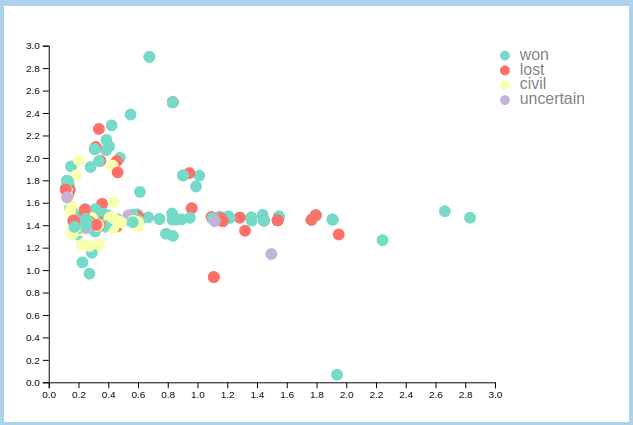
\includegraphics[scale=0.30]{./images/scatter_plot.png}
    \caption{Scatter plot}
\end{figure}
The scatter plot is one more component of our dashboard, used to represent the roman battles after a dimensionality reduction on two dimensions.

In particular, this chart represents the first two components, $y_1$ and $y_2$, obtained after the execution of a static MCA on the battles. This chart allows the user to:
\begin{itemize}
    \item find similar events, taking into account the distance between the points
    \item individuating clusters
    \item discover outliers
\end{itemize}

We have decided to add a chromatic encoding of the points, associating to each color a different outcome: the colors are the same used in the geographic map.

The user is also given the possibility to brush a zone of interest on the graph: the points within the zone are highlighted in the geographic map as well.

\subsection{Filters - Header}
\begin{figure}[h]
    \centering
    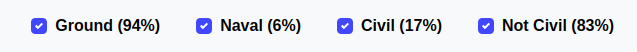
\includegraphics[scale=0.32]{./images/header_filters.png}
    \caption{Header filters}
\end{figure}
Another main component of our project is the header. Indeed, in order to allow the analyst to further customize its analysis, we decided to implement a set of simple filters such as \textbf{Ground}, \textbf{Naval}, \textbf{Civil} and \textbf{Not Civil}. By default, all filters are selected, i.e. the whole dataset is visualized. The activation (resp. deactivation) of a filter triggers a function that hides (resp. shows) all the data corresponding to that filter.

\subsection{Dark and blind safe modes}
Other additional features available in our visualization to allow the analyst to feel comfortable are the \textbf{dark theme} and \textbf{blind safe mode}. We decided to introduce the first one, since a human in different time periods of the day can be mentally tired, and couldn't pay so much attention to several visualization information. In order to reduce this issue, we decided to provided a more relaxing colors combination for the eyes, thanks to \href{https://colorbrewer2.org/}{ColorBrewer} web tool \cite{HB03}. The default theme is the light one, which uses a colors combination brighter and lighter with respect to the one used for the dark theme. Another problem that could arise is referred to the colorblind people. In fact, these people see particular colors in different ways, for example a green color can be seen as brown one. For this reason, we decided to introduce also a blind safe mode, always supported by ColorBrewer, which uses a colors combination that have been scientifically chosen in order to reduce the confusion likelihood as much as possible.

We want to underline that we have used the same blind safe colors combination for both themes.